% =====================================================================
% Project process report: what was done, why, and how, independent of
% the paper's own narrative. Intended as a standalone technical record
% (methodology diary), not for journal submission.
%
% Compile with: pdflatex PROJECT_PROCESS_REPORT.tex (run twice for refs)
% =====================================================================
\documentclass[11pt]{article}

\usepackage[a4paper,margin=2.2cm]{geometry}
\usepackage{amsmath,amssymb}
\usepackage{graphicx}
\usepackage{xcolor}
\usepackage{booktabs}
\usepackage{hyperref}
\usepackage{tikz}
\usetikzlibrary{arrows.meta,positioning,shapes.geometric,fit,backgrounds,calc}

\title{\textbf{Project Process Report:}\\
HAPS/UAV Channel Model, Rain-Attenuation LSTM, and DQN Association Agent}
\author{Process diary -- methodology, diagnostics, and modeling decisions}
\date{\today}

\newcommand{\block}[4]{\node[draw, rounded corners, fill=#4, minimum width=3.1cm, minimum height=1cm, align=center, font=\small] (#1) at #2 {#3};}

\begin{document}
\maketitle

\tableofcontents

% =====================================================================
\section{Purpose of this document}
% =====================================================================
The paper reports results; it does not explain the process that produced them. This
document is the process record: what was attempted, what broke, how each problem was
diagnosed (not just stated), and the modeling decisions behind the DQN's MDP and the
LSTM's training protocol. It is written for whoever needs to reproduce, extend, or
defend this work later (including ourselves, months from now), not for a journal
reviewer.

% =====================================================================
\section{End-to-end pipeline}
% =====================================================================
Three subsystems feed into each other in a fixed order: the channel model produces
geometry and SINR; the LSTM forecasts rain attenuation from historical weather; the
DQN consumes both to learn an association policy. A change anywhere upstream
invalidates everything downstream -- this is the reason the UAV-relay geometry fix
(\S\ref{sec:uav-bug}) forced a full DQN retrain, and the LSTM retrain
(\S\ref{sec:overfitting}) forced a forecast and episode regeneration before the DQN
could be rerun again.

\begin{center}
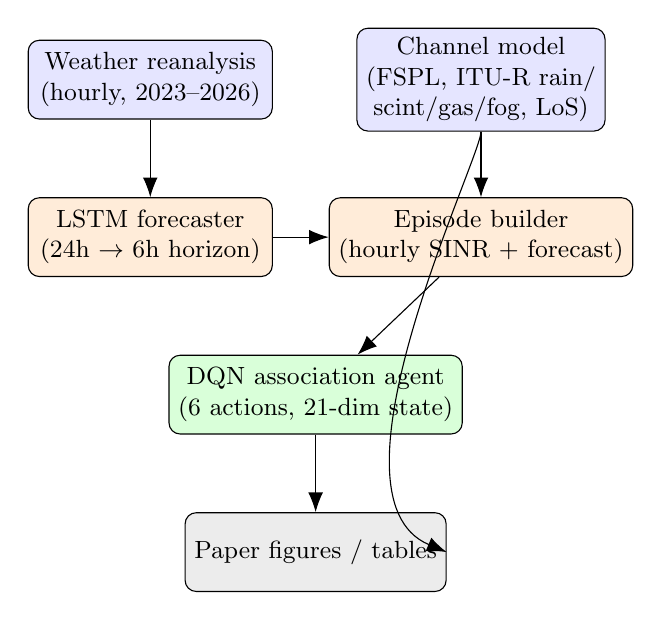
\begin{tikzpicture}[node distance=0.9cm, >={Latex[length=2.5mm]}]
\block{weather}{(0,0)}{Weather reanalysis\\(hourly, 2023--2026)}{blue!10}
\block{channel}{(4.2,0)}{Channel model\\(FSPL, ITU-R rain/\\scint/gas/fog, LoS)}{blue!10}
\block{lstm}{(0,-2)}{LSTM forecaster\\(24h $\to$ 6h horizon)}{orange!15}
\block{episodes}{(4.2,-2)}{Episode builder\\(hourly SINR + forecast)}{orange!15}
\block{dqn}{(2.1,-4)}{DQN association agent\\(6 actions, 21-dim state)}{green!15}
\block{paper}{(2.1,-6)}{Paper figures / tables}{gray!15}

\draw[->] (weather) -- (lstm);
\draw[->] (channel) -- (episodes);
\draw[->] (lstm) -- (episodes);
\draw[->] (episodes) -- (dqn);
\draw[->] (dqn) -- (paper);
\draw[->] (channel.south) .. controls (4.2,-1) and (2.1,-5.3) .. (paper.east);
\end{tikzpicture}
\end{center}

% =====================================================================
\section{The UAV-relay geometry bug}
\label{sec:uav-bug}
% =====================================================================

\subsection{Problem statement}
The original relay model placed the single relay UAV \emph{adjacent to whichever user
it was currently serving} -- i.e.\ the UAV's position was a function of the user being
evaluated, re-derived per user, per timestep. This is physically backwards: a real UAV
occupies one position at a time; it cannot simultaneously hover next to every user it
might serve. The bug was caught by inspecting \texttt{haps\_association\_env.py}'s
relay-capacity call and noticing the horizontal distance argument was the user's own
distance to its serving HAPS, not a UAV-specific distance at all -- the UAV was not a
separate entity in the geometry, just a relabeling of the direct link.

\subsection{Consequence}
Because the UAV silently tracked every user, relay actions never actually degraded with
distance the way a real feeder+access path would. The DQN, trained on this geometry,
learned to over-use relay actions that would not survive a real deployment, and every
downstream relay-related number (Fig.~12, the relay-path section, the DQN's action
distribution) was describing a physically unrealizable system.

\subsection{Fix}
A single relay UAV was fixed at the centroid of the HAPS triangle (circumradius
$65/\sqrt{3}\approx37.5$\,km from each HAPS, giving a constant feeder-hop elevation of
$\approx27.5^\circ$ and a flat feeder capacity of 10.2\,bits/s/Hz for every HAPS, by the
constellation's symmetry). The access hop (UAV$\to$UE) now uses the user's \emph{real}
distance to that fixed point, so capacity collapses realistically with distance --
usable radius $\approx6.5$\,km before capacity drops below 0.5\,bits/s/Hz.

\begin{center}
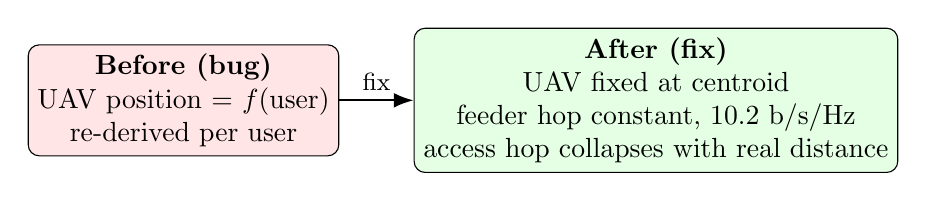
\begin{tikzpicture}[>={Latex[length=2.5mm]}]
\node[draw, fill=red!10, rounded corners, align=center] (bugL) at (0,0) {\textbf{Before (bug)}\\UAV position = $f$(user)\\re-derived per user};
\node[draw, fill=green!10, rounded corners, align=center] (fixR) at (6,0) {\textbf{After (fix)}\\UAV fixed at centroid\\feeder hop constant, 10.2 b/s/Hz\\access hop collapses with real distance};
\draw[->, thick] (bugL) -- node[above]{\small fix} (fixR);
\end{tikzpicture}
\end{center}

\subsection{Why this forced a full retrain}
Three of the DQN's six actions (the relay options) changed meaning entirely -- from
"always nearly free" to "usually a trap beyond 6.5\,km." A policy trained under the old
geometry had learned action values that no longer corresponded to real outcomes, so
retraining (not just re-evaluating) was mandatory.

% =====================================================================
\section{DQN undertraining diagnosis}
% =====================================================================
After the geometry fix, the DQN's reward was noticeably worse and noisier than before.
Rather than accept this as "the fix made things worse," a controlled diagnostic was run:
reward-vs-episode curves were plotted for a longer training budget. Reward was still
visibly climbing, not plateaued, at 1600 of the original 400-episode-equivalent budget.
This ruled out "the new geometry is just harder to learn" (which would plateau early at
a lower level) in favor of "the agent needs more experience to re-learn which of its six
actions are now traps." Training budget was increased from 400 to 2400 episodes (the
400 real 2024 episodes cycled six times), across 10 random seeds (up from 5) for
statistical power.

% =====================================================================
\section{LSTM overfitting diagnosis}
\label{sec:overfitting}
% =====================================================================

\subsection{Symptom}
The original LSTM (30 training epochs, no held-out validation set) showed training loss
monotonically decreasing for all 30 epochs -- the textbook shape of a model that is
still being told to fit, with no signal telling it when to stop.

\subsection{Diagnosis: a proper three-way split}
A validated train/validation/test split was introduced, strictly chronological so no
future information leaks backward:

\begin{center}
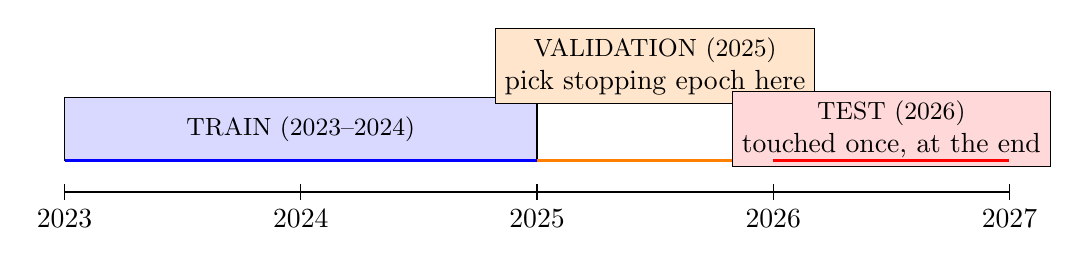
\begin{tikzpicture}[>={Latex[length=2.5mm]}]
\draw[thick] (0,0) -- (12,0);
\foreach \x/\lbl in {0/2023, 3/2024, 6/2025, 9/2026, 12/2027} {
  \draw (\x,0.1) -- (\x,-0.1);
  \node[below] at (\x,-0.1) {\lbl};
}
\node[draw, fill=blue!15, minimum height=0.8cm, minimum width=6cm, align=center] at (3,0.8) {\small TRAIN (2023--2024)};
\draw[thick,blue] (0,0.4) -- (6,0.4);
\node[draw, fill=orange!20, minimum height=0.8cm, minimum width=3cm, align=center] at (7.5,1.6) {\small VALIDATION (2025)\\pick stopping epoch here};
\draw[thick,orange] (6,0.4) -- (9,0.4);
\node[draw, fill=red!15, minimum height=0.8cm, minimum width=3cm, align=center] at (10.5,0.8) {\small TEST (2026)\\touched once, at the end};
\draw[thick,red] (9,0.4) -- (12,0.4);
\end{tikzpicture}
\end{center}

The model was trained up to 100 epochs, checking validation RMSE every 2 epochs and
keeping the checkpoint at the \emph{best validation epoch} -- never the test set. Result:
best epoch was 4 (val RMSE 0.738), with validation RMSE degrading steadily afterward --
confirming overfitting was real and quantifying exactly where it started, rather than
guessing a round number like "10 epochs should be safe."

\subsection{A real bug found while diagnosing}
The first version of this early-stopping script produced all-NaN aggregate metrics.
Root cause: 2026's weather data has $\approx$139\,NaN rows from data gaps, and
\texttt{make\_windows} did not filter windows touching a NaN -- \texttt{np.mean} over an
array containing even one NaN returns NaN, silently poisoning every aggregate. Fixed by
filtering any window whose input or target touched a NaN before computing metrics,
matching the convention already used elsewhere in the codebase
(\texttt{export\_lstm\_forecasts.py}).

\subsection{Propagating the fix to all three checkpoints}
The DQN pipeline depends on three separately-trained LSTM checkpoints, each with a
different training-year convention (to keep every forecast genuinely out-of-sample for
the data it is applied to):

\begin{center}
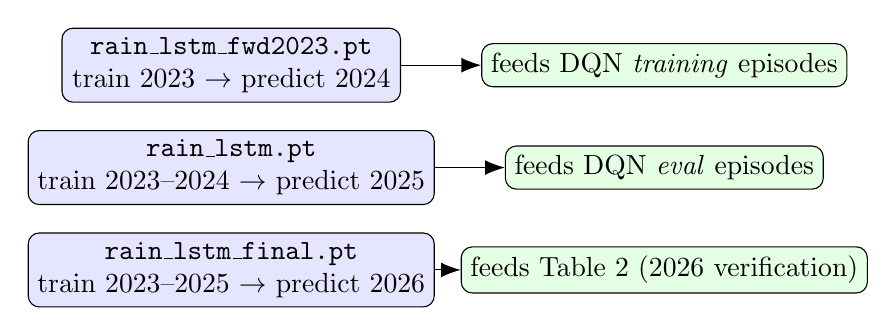
\begin{tikzpicture}[>={Latex[length=2.5mm]}, node distance=0.6cm]
\node[draw, fill=blue!10, rounded corners, align=center, minimum width=4.3cm] (m1) at (0,0) {\texttt{rain\_lstm\_fwd2023.pt}\\train 2023 $\to$ predict 2024};
\node[draw, fill=blue!10, rounded corners, align=center, minimum width=4.3cm] (m2) at (0,-1.3) {\texttt{rain\_lstm.pt}\\train 2023--2024 $\to$ predict 2025};
\node[draw, fill=blue!10, rounded corners, align=center, minimum width=4.3cm] (m3) at (0,-2.6) {\texttt{rain\_lstm\_final.pt}\\train 2023--2025 $\to$ predict 2026};
\node[draw, fill=green!10, rounded corners, align=center, minimum width=4cm] (use1) at (5.5,0) {feeds DQN \emph{training} episodes};
\node[draw, fill=green!10, rounded corners, align=center, minimum width=4cm] (use2) at (5.5,-1.3) {feeds DQN \emph{eval} episodes};
\node[draw, fill=green!10, rounded corners, align=center, minimum width=4cm] (use3) at (5.5,-2.6) {feeds Table 2 (2026 verification)};
\draw[->] (m1) -- (use1); \draw[->] (m2) -- (use2); \draw[->] (m3) -- (use3);
\end{tikzpicture}
\end{center}

All three were retrained at \texttt{EPOCHS=4} (the validated stopping point), and every
downstream artifact was regenerated in order: forecasts
(\texttt{export\_lstm\_forecasts.py}) $\to$ Fig.~8 (\texttt{plot\_forecast\_windows.py})
$\to$ DQN episodes (\texttt{build\_real\_episodes.py}) $\to$ DQN retrain
(\texttt{run\_multiseed.py}, \texttt{run\_ablations.py}, \texttt{run\_baselines\_5seed.py}).

One mistake worth recording: retraining \texttt{rain\_lstm.pt} with
\texttt{-{}-years 2023 2024} trained on 2023 \emph{only}, because
\texttt{train\_lstm.py}'s internal chronological split treats the \emph{last} listed
year as the held-out test year. The fix was \texttt{-{}-years 2023 2024 2025}, making
2023+2024 the combined training set and 2025 the internal test year -- verified correct
by matching the resulting RMSE (0.7380) against the Stage-1 validation result.

% =====================================================================
\section{Ensembling plan}
% =====================================================================
Once the LSTM was properly early-stopped, the question became whether blending it with
a trivial persistence baseline (``tomorrow looks like today'') could improve on either
alone. The chosen protocol, deliberately designed to avoid any test-set leakage:

\begin{enumerate}
  \item For each forecast horizon ($h=1,\dots,6$ hours) independently, sweep a blend
  weight $w\in[0,1]$ on the LSTM (and $1-w$ on persistence).
  \item Pick the $w$ that minimizes RMSE on the \textbf{validation} set (2025) only.
  \item Apply that fixed, per-horizon $w$ once to the \textbf{test} set (2026) and report
  the result -- the test set is never used to choose $w$.
\end{enumerate}

Result: the optimal weight was $\approx1.0$ (essentially all-LSTM) at every horizon
except $+1$\,h, where persistence gets partial weight ($w\approx0.75$) -- consistent with
persistence being hard to beat at the very shortest horizon (little has changed in an
hour) but losing ground quickly as the horizon grows and the LSTM's learned dynamics
matter more.

% =====================================================================
\section{DQN MDP modeling}
% =====================================================================

\subsection{Per-user formulation}
Each user is modeled as an independent Markov decision process, re-solved at every
hourly timestep:

\begin{center}
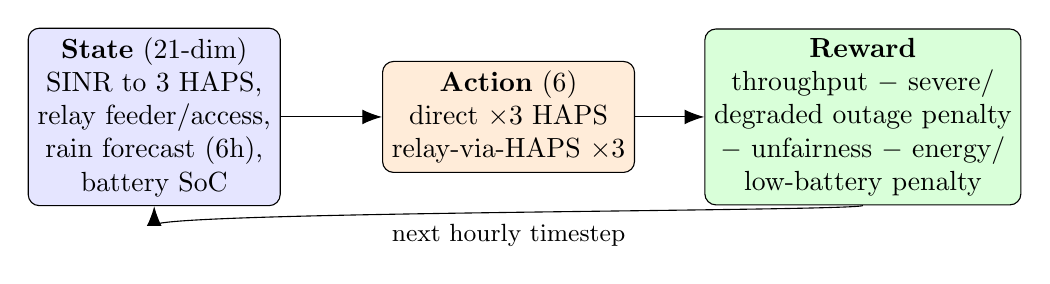
\begin{tikzpicture}[>={Latex[length=2.5mm]}]
\node[draw, fill=blue!10, rounded corners, minimum width=3.2cm, align=center] (state) at (0,0) {\textbf{State} (21-dim)\\SINR to 3 HAPS,\\relay feeder/access,\\rain forecast (6h),\\battery SoC};
\node[draw, fill=orange!15, rounded corners, minimum width=3.2cm, align=center] (action) at (4.5,0) {\textbf{Action} (6)\\direct $\times$3 HAPS\\relay-via-HAPS $\times$3};
\node[draw, fill=green!15, rounded corners, minimum width=3.2cm, align=center] (reward) at (9,0) {\textbf{Reward}\\throughput $-$ severe/\\degraded outage penalty\\$-$ unfairness $-$ energy/\\low-battery penalty};
\draw[->] (state) -- (action);
\draw[->] (action) -- (reward);
\draw[->] (reward.south) .. controls (9,-1.2) and (0,-1.2) .. (state.south);
\node at (4.5,-1.5) {\small next hourly timestep};
\end{tikzpicture}
\end{center}

\subsection{Why relay is folded into one per-user choice (for now)}
With a single, fixed-position UAV, "which HAPS feeds the UAV" is not yet a real decision
-- there is only one UAV and one centroid. So relay-vs-direct could be collapsed into one
flat six-way choice per user without losing any real degrees of freedom. This
simplification breaks once multiple UAVs are introduced: UAV-to-HAPS assignment becomes
its own $O(\text{fleet size})$ problem, decoupled from the $O(N)$ per-user access
decision, and relay-vs-direct would need to become an explicit policy layer rather than
one branch of a single per-user action set (flagged as future work, not yet implemented).

\subsection{Statistical validation protocol}
Every comparison in the paper (DQN vs.\ baselines, forecast ablation) uses the same
discipline: train $N$ independent seeds, evaluate all variants on the \emph{same}
held-out days, and report paired differences (not independent-sample tests, since the
same evaluation days are shared across policies within a seed) with a paired $t$-test
and the fraction of seeds where one variant beats another. The $\alpha=0.05$ convention
is used throughout; a $p$-value \emph{between} two non-standard cutoffs (e.g.\ "$p>0.02$")
was caught in self-review as a misleading nonstandard framing and corrected everywhere it
appeared.

% =====================================================================
\section{Files modified and commands run}
% =====================================================================
This section is the literal record: which files were edited or created, and the exact
command used to run each stage. Paths are relative to the repository root; all commands
were run from WSL with the \texttt{quantum\_env} environment active unless noted.

\subsection{UAV-relay geometry fix (\S\ref{sec:uav-bug})}
\begin{itemize}
  \item \texttt{src/drl\_dqn/haps\_association\_env.py} -- modified. Relay-capacity call
  changed from the user's own HAPS distance to a fixed per-HAPS centroid distance
  (\texttt{self.uav\_xy\_m}) for the feeder hop, and the real UAV--UE distance for the
  access hop.
  \item \texttt{src/generators/generate\_uav\_relay\_table.py} -- modified, to sweep
  azimuth-averaged distance from the serving HAPS under the fixed-centroid geometry.
  \begin{verbatim}
python src/generators/generate_uav_relay_table.py
  \end{verbatim}
  \item \texttt{src/generators/generate\_uav\_placement\_study.py} -- created: single-UAV
  radial sweep plus a covering-number calculation for full-coverage UAV fleet size.
  \begin{verbatim}
python src/generators/generate_uav_placement_study.py
  \end{verbatim}
\end{itemize}

\subsection{DQN retrain, 400\,$\to$\,2400 episodes, 5\,$\to$\,10 seeds}
\begin{itemize}
  \item \texttt{src/drl\_dqn/run\_multiseed.py} -- modified:
  \texttt{N\_TRAIN\_EPISODES = 2400}, \texttt{SEEDS = [0..9]}.
  \item \texttt{src/drl\_dqn/run\_ablations.py} -- same two changes.
  \item \texttt{src/drl\_dqn/plot\_seed\_and\_paired.py} -- modified: replaced hardcoded
  seed counts in titles/labels with \texttt{len(dqn)}, computed dynamically.
  \item \texttt{src/drl\_dqn/run\_reward\_decomposition.py} -- created: retrains the same
  5 seeds, adds per-reward-term decomposition (throughput/severe/degraded/fairness/
  energy/low-battery) not carried by the main multiseed output.
  \item \texttt{src/drl\_dqn/run\_relay\_targeting\_check.py} -- created: checks whether
  relay usage targets poor-SINR users and correlates with the rain forecast, with
  per-seed incremental CSV writes and significance tests.
  \begin{verbatim}
python src/drl_dqn/run_multiseed.py
python src/drl_dqn/run_baselines_5seed.py
python src/drl_dqn/run_ablations.py
python src/drl_dqn/run_reward_decomposition.py
python src/drl_dqn/run_relay_targeting_check.py
python src/drl_dqn/plot_seed_and_paired.py
  \end{verbatim}
\end{itemize}

\subsection{LSTM overfitting diagnosis and retrain (\S\ref{sec:overfitting})}
\begin{itemize}
  \item \texttt{src/lstm/train\_lstm.py} -- unmodified (reference implementation of
  \texttt{RainLSTM}, \texttt{make\_windows}, \texttt{build\_table}), but invoked directly
  via CLI to retrain \texttt{rain\_lstm.pt}:
  \begin{verbatim}
python src/lstm/train_lstm.py --years 2023 2024 2025 --epochs 4
  \end{verbatim}
  (\texttt{2023 2024 2025}, not \texttt{2023 2024} -- the script's internal split treats
  the \emph{last} listed year as the held-out test year, so three years are needed to
  make 2023+2024 the combined training set and 2025 the test year.)
  \item \texttt{src/lstm/train\_lstm\_earlystop.py} -- created: honest
  train(2023--2024)/validation(2025)/test(2026) split, up to 100 epochs, validation RMSE
  checked every 2 epochs, best-validation-epoch checkpoint saved. Found best epoch~=4.
  \begin{verbatim}
python src/lstm/train_lstm_earlystop.py
  \end{verbatim}
  \item \texttt{src/lstm/train\_forward\_lstm.py} -- modified: \texttt{EPOCHS = 30}
  $\to$ \texttt{EPOCHS = 4}.
  \begin{verbatim}
python src/lstm/train_forward_lstm.py
  \end{verbatim}
  \item \texttt{src/lstm/train\_final\_lstm.py} -- modified: \texttt{EPOCHS = 30}
  $\to$ \texttt{EPOCHS = 4}.
  \begin{verbatim}
python src/lstm/train_final_lstm.py
  \end{verbatim}
  \item \texttt{src/lstm/ensemble\_weighted.py} -- created: per-horizon weight sweep on
  the 2025 validation set, applied once to the 2026 test set.
  \begin{verbatim}
python src/lstm/ensemble_weighted.py
  \end{verbatim}
\end{itemize}

\subsection{Regenerating everything downstream of the LSTM retrain}
Run strictly in this order -- each step's output feeds the next:
\begin{itemize}
  \item \texttt{src/lstm/export\_lstm\_forecasts.py} -- unmodified, rerun to regenerate
  \texttt{data/processed/lstm/lstm\_dqn\_inputs.csv} from the three retrained checkpoints.
  \item \texttt{src/lstm/plot\_forecast\_windows.py} -- unmodified, rerun (this is Fig.~8's
  actual generator, reading \texttt{lstm\_dqn\_inputs.csv}).
  \item \texttt{src/drl\_dqn/build\_real\_episodes.py} -- unmodified, rerun to rebuild
  \texttt{data/processed/episodes/episodes\_hourly.csv} with the new forecast columns.
  \begin{verbatim}
python src/lstm/export_lstm_forecasts.py
python src/lstm/plot_forecast_windows.py
python src/drl_dqn/build_real_episodes.py
  \end{verbatim}
  then rerun the full DQN stage (previous subsection) again, since the episodes changed.
\end{itemize}

% =====================================================================
\section{Verification discipline}
% =====================================================================
The practice that caught most of the real bugs above: never trust a script's printed
summary number without independently recomputing it from the raw per-seed/per-window
output at least once. This caught the NaN-propagation bug (aggregate metrics printed as
NaN, root cause only visible by inspecting window-level data), the wrong
\texttt{-{}-years} flag (caught by cross-checking RMSE against an independently-computed
reference), and a mis-bolded "best" value in an early table draft (caught by resorting
the raw numbers instead of trusting which cell had been bolded).

\end{document}
